%!TEX root=../robocert.tex
\begin{figure}
	\centering
	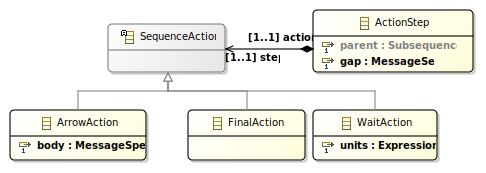
\includegraphics[width=0.7\textwidth]{diagrams/Actions}
	\caption{Class diagram for the part of the \langname{} metamodel dealing with actions.}
	\label{fig:metamodel-actions}
\end{figure}

\Cref{fig:metamodel-actions} depicts the part of the metamodel concerning
sequence actions.

A \msequenceaction{} is an explicit communication or control flow construct in a
\msubsequence.  There are currently three types of action: arrow, loop, and
final actions.

\subsection{\marrowaction}

An \marrowaction\footnote{The name signifies both that the actions resemble
PSC \emph{arrowMSG} specifications, and also that they correspond to arrows in
the graphical syntax.} specifies one communication between \mactor s which is on
the sequence specified by the diagram.  Each \marrowaction{} wraps one
\marrowmessagespec{} (\cref{sec:metamodel-messages})
containing the specification proper.
\todo{Eventually these will bind arguments.}

\begin{figure}[h]

\begin{subfigure}[t]{0.38\textwidth}
\begin{lstlisting}[style=Example]
-> operation O1()
\end{lstlisting}
\end{subfigure}
\hfill
\begin{subfigure}[t]{0.58\textwidth}
\gsecaption
\centering
\begin{tikzpicture}
\matrix[diagram]{
    \node[rcmodule](mstart) {\egtarget}; & \node[world](wstart) {\egworld}; \\
	\coordinate(mo); & \coordinate(wo); \\
	\coordinate(mend); & \coordinate(wend); \\
};
\draw[lifeline] (mstart) -- (mo) -- (mend);
\draw[lifeline] (wstart) -- (wo) -- (wend);
\draw (mo) edge[oarrow, "O1()"] (wo);
\end{tikzpicture}
\end{subfigure}

\end{figure}

\subsection{\mloopaction}

A \mloopaction{} is a \emph{named} infinite loop.  \todo{Breaking and perhaps
other forms of loop are forthcoming.}  Each \mloopaction{} contains one
\msubsequence{} of steps to repeat indefinitely.

\begin{lstlisting}[style=Example]
loop L {
    -> operation O2()  // Subsequence
}  // infinite LoopAction
\end{lstlisting}

\subsection{\mfinalaction}

A \mfinalaction{} captures the successful termination of a sequence diagram.
A diagram with a \mfinalaction{} specifies a complete sequence of behaviour
from the \mtarget{} initialising to the \mtarget{} terminating.  Conversely,
sequence diagrams without \mfinalaction s capture partial specifications of
behaviour, or the behaviour of \mtarget s that do not terminate.

Note that the final \msequencegap{} before a \mfinalaction{} captures
any permitted communications after the behaviour explicitly specified by the
diagram has occurred.

\begin{figure}[h]

\begin{subfigure}[t]{0.38\textwidth}
\begin{lstlisting}[style=Example]
end
\end{lstlisting}
\end{subfigure}
\hfill
\begin{subfigure}[t]{0.58\textwidth}
\gsecaption
\centering
\begin{tikzpicture}
\matrix[diagram]{
	\node[rcmodule](mstart) {\egtarget}; & \node[world](wstart) {\egworld}; \\
	\coordinate(mend); & \coordinate(wend); \\
};
\draw[lifeline] (mstart) -- (mend);
\draw[lifeline] (wstart) -- (wend);
\draw (mend) edge[final] (wend);
\end{tikzpicture}
\end{subfigure}

\end{figure}

%%% Local Variables:
%%% mode: latex
%%% TeX-master: "../robocert"
%%% End:
